\section{The Project}
It is believed that computers may perform better in many settings if they are able to determine the meaning of a text. There are different ways of achieving this result, and one of them is by automatic content categorization. Automatic content categorization is a process where the text is categorized to the most describing category from a set of desirable categories. There are various ways of performing automatic content categorization. This project focuses on categorizing text based on which keywords occur in the text and these keywords' categories. 
%The approach for this consists of finding relevant keywords and desirable categories, create a mapping between the keywords and the categories, and then determine the most likely category for the text based the keyword occurrences. 

\begin{figure}[h]
\centering
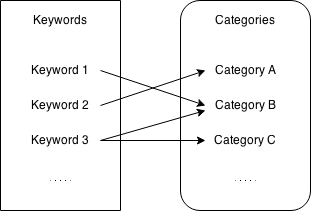
\includegraphics[width=0.65\textwidth]{Chapters/Introduction/keywordstocategories}
\caption{Illustration of the mapping between keywords and categories.}
\label{fig:keywordstocategories}
\end{figure}


Creating this automatic content categorization consists of three main steps. The first step is to create a list of keywords and a set of desirable categories for the categorization process. For this project have we chosen the keywords to be titles of Wikipedia articles, and taxonomy from  \emph{Interactive Advertising Bureau} (IAB) taxonomy as the set of desirable categories. 
%The Wikipedia article titles need be processed before they can be used as keywords and some changes might be necessary to create a 
Both Wikipedia article titles and IAB's taxonomy need to be processed before they are suitable as keywords and category set. 

The next step is creating a mapping between the keywords and the categories (see figure \ref{fig:keywordstocategories}). This step takes advantage of the underlying structure of Wikipedia to find the meaning of the Wikipedia article so that the keywords map to categories describing their content.

The final step of the categorization process is determining the category of any given text. Figure \ref{fig:categorizetext} shows this process, where all keywords are found in the given text and the text's category is determined from the keywords' categories. It is also essential to use some technique for finding keywords in the text, and this project has used software from Cxense for this step. 

\begin{comment}

Example of a categorization could be the simple collection of the two texts: $t_{1}$ = \emph{Zlatan and Messi play soccer} and $t_{2}$ = \emph{The sun in yellow}.  \emph{soccer}, \emph{Messi} and \emph{Zlatan} are keywords mapping to the category \emph{Sports/soccer}

As example should an article which contains the words \emph{soccer}, \emph{Messi} and \emph{Zlatan} should probably be categorized as \emph{Sports/Soccer} if these are available keywords mapped to this category.  


\end{comment}
%nderstanding text is important for 
%utomatic content categorization is useful for determining the meaning of a text which is useful in many settings. 
%Given a set of desirable categories it
%To be able to categorize articles, it is 
%Thus our overall goal is defined as creating a classifier that maps keywords from a predefined keyword list and to one or more pre-defined categories. The automatic categorization will include both the creation of the predefined keyword list and the mapping function, which are both essential for categorizing collections of texts based on their content. 

%Creating this automatic content categorization consists of *** steps. the first step is to find all keywords 


\begin{figure}[h]
\centering

\includegraphics[width=\textwidth]{Chapters/Introduction/categorizetext}
\caption{Simplified illustration of the categorization process.}
\label{fig:categorizetext}
\end{figure}

\begin{comment}
\begin{figure}[H]
\centering
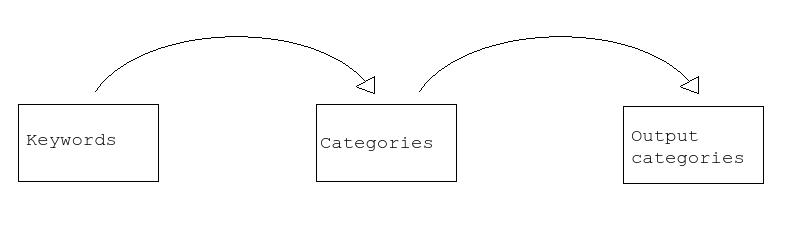
\includegraphics[width=1\textwidth]{Chapters/Introduction/classification_process.jpeg}
\caption{A simplified illustration of the categorization process.}
\label{fig:classification_process}
\end{figure}
\end{comment}
%This classifier will be used as part of an automatic categorization process. 
%Our overall goal is therefore to make an automatic categorization that have a predefined keyword list and start by creating a mapping from each keyword to a category from another predefined list. Where the category of a text can be defined from the keywords found in the text. 

\section{An Overview of Challenges}
This project has encountered some challenges within different fields. Some of the challenges were solved better than others. 

\subsubsection{Representing the Structure}
The structure of Wikipedia is found in multiple files containing lots of information. The underlying structure is quite complex, and is poorly documented from a developer's point of view. The first challenge encountered was deciding the information required for representing the structure and determining a suitable structure for the representation.



\begin{comment}
The main challenges encountered had to do with Wikipedia, mainly because the encyclopedia is maintained by thousands of volunteers and is poorly documented from a developer's point of view. The structure of Wikipedia is complex and the size makes it hard to check if the results found are correct. 

\end{comment}

%which also leads to a complicated and complex structure. 

\subsubsection{Encoding}
Wikipedia is available in multiple languages and is written by volunteers from all over the world. This makes Wikipedia a multilingual encyclopedia with knowledge available from everywhere and it is possible for experts form various fields and from different parts of the world to contribute with knowledge. There are both advantages and disadvantages with a multilingual encyclopedia. One of the disadvantages is that users might write with different encoding (e.g. \emph{utf8}, \emph{ascii} or \emph{unicode}). Problems occur when going through all the names of Wikipedia categories and Wikipedia article titles because titles written in different encoding might not be viewed as identical by the computer. 

An example of a category name which leads to trouble with encoding is  \emph{Communes in Cara\cb{s}-Severin County}, which is either written with the letter \emph{\cb{s}} \cite{swithcomma} or \c{s} \cite{swithcedilla}. These letters are examples of characters that makes matching category names difficult, because \emph{Communes in Cara\cb{s}-Severin County} and \emph{Communes in Cara\c{s}-Severin County} will not be equal to the computer even though it is clear to most users that they should be the same. 

This problem was partly solved by changing all category names and article titles to the same encoding by transforming all text to \emph{utf-8}, including escape of \emph{unicode} characters with \cite{unidecode}. This solved most of the problem, but some category names did not become equal even though most humans would consider them equal. A total of 10800 categoroies was not able to be matched out of \textbf{INSERT NUMBER}. These categories represent a very small part of all categories  (equivalent to 0.9\%), and were therefore disregarded. 


\subsubsection{Disambiguation}
Antoher problem encountered is disambiguation. Wikipedia contains many titles that could have various meanings (see figure \ref{fig:disambiguation_example}). This means that the titles is ambiguous and leads to the common problem in natural language processing: disambiguation \cite{wiki:disambiguation}. A complete section (\ref{sec:disambiguation}) is dedicated to different solutions to this specific problem. 
%others work within in the topic see \ref{sec:disambiguation}

\begin{figure}[h]
\centering
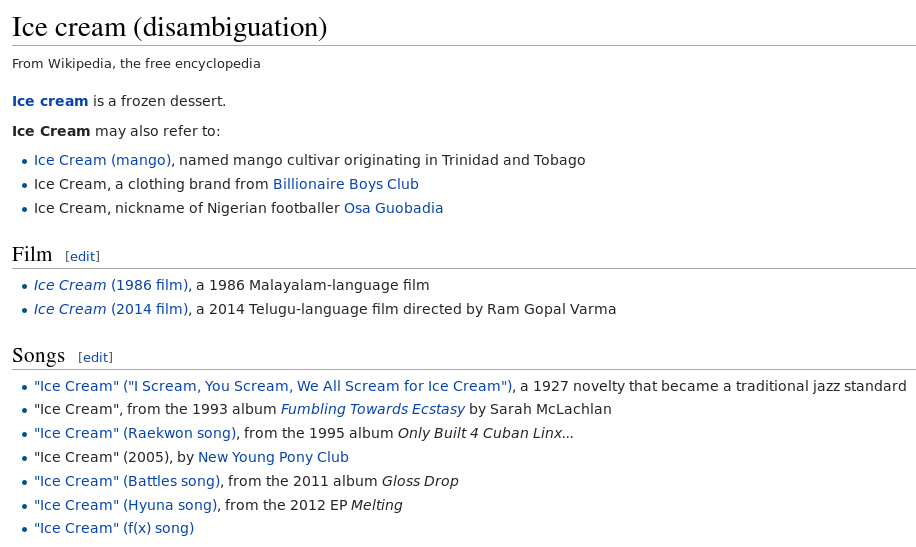
\includegraphics[width=\textwidth]{Chapters/Introduction/Ice_cream_disambiguation}
\caption{Example of disambiguation in Wikipedia \cite{wiki:icecreamdisambiguation}.}
\label{fig:disambiguation_example}
\end{figure}